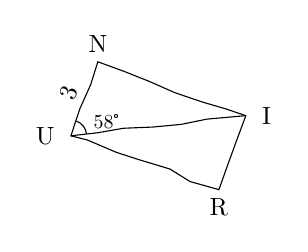
\begin{tikzpicture}[rotate=-20,every node/.style={scale=0.9},scale=1]

\coordinate (U) at (0,0);
\coordinate (N) at (0,1);
\coordinate (I) at (2,1);
\coordinate (R) at (2,0);

\draw[decorate,decoration={random steps,amplitude=1pt,segment length=10pt}] (U) node [left=3pt]{U}--(N) node [above]{N}--(I) node [right=3pt] {I}--(R) node [below] {R}--cycle;
\draw [decorate,decoration={random steps,amplitude=1pt,segment length=10pt}] (U)--(I);
\path (U)--(N) node[midway,above,rotate=70]{3};
\draw (0,0.2) arc (90:26.57:0.2) node[above=5pt,right,scale=0.8]{58°};

\end{tikzpicture}